%Student record/marks system
%Backend Documentation by Masana Khosa (559990) and Londiwe Ngema (448871)

\section{Part A : Front-end}

This section presents the design of the user interface of the software. The user interface provides a visual platform for all the users. It provides a more user friendly environment to the client's database queries. The users are able to read and write from and into the database through the user interface. The user interface was implemented using HTML, JavaScript, CSS, and PHP. HTML was used for designing attributes or objects on user interface platforms. JavaScript was used for the animations on the welcome page. CSS gives application its custom look. PHP was used to help users query the database through the user interface. 

The user interface consist of a login page. In the login page, all the users will be asked to input login details and that includes the user-name, password and domain. The login details will be queried into the database to see if they are valid. If the login details are not valid, an error message will be displayed to the user. If the login in details are valid, the user will be redirected to a specific page according to the specified domain. If the user is a course coordinator, the user will be redirected to a course coordinator page, if the user is an administrator, the user will be to an administrator page and same applies for the student. The page where a user will be redirected to depends on the domain specified. Each page where users will be redirected to has a logout button that takes the user back to the login home page. 


\subsection{Login page design}

HTML: Different HTML tags used to describe HTML documents were used to describe the login page. The login page consists of the welcome text and wits pictures to create a more attractive but simple welcome page. A form with input tags for users to input the user-name and password was placed on the login page. The form also consist of a drop-down tag to select the domain. A submit button was also placed to submit the form with login details.

CSS: A CSS file was made for the home page. All the tags mentioned above were given an "id" which is used for reference in the CSS file. In the CSS file for the login page, each tag was given a position, colour, opacity, background colour and all the other styling necessary. 

JavaScript: When the login page is opened, a welcome title slides in from the left of the page up until the middle of the page, when the welcome tittle is done sliding, a wits logo is displayed behind the welcome statement. All theses animations of objects on the login page were done using JavaScript.    

     
PHP: PHP receives the posted form that has the login details of a specific user after when the user presses the submit button. The login details in the form are then sent to the database for verification. If the login details are valid, the user is then redirected to either a student page, course co-ordinator page or administrator page depending on the domain specified.   

\subsection{Student page design}

HTML: The student page was designed to be more user friendly. The student page consists of a menu section where the student can select the options based on their level of access. All the options in the menu section are hypertext references that redirect the student to a specific page based on the selected option. Adjacent to the menu section is a 'more-information' section that explains in detail what each of the menu options is for.

The options in the menu section are:-

\begin{itemize}
\item Assessment marks for a course
\item Statistics
\item Assessment  marks for all courses
\item Performance goals
\end{itemize} 


CSS: The styling of each attribute on the student page was defined on the CSS file.

PHP: When each of the hypertext references in the menu section is clicked, the student is redirected to a specific page depending on the option chosen. When a student selects assessment marks for all courses option, his/her student number will be used to query a table with final marks associated with that student number and the final marks for each course will be displayed to the student. When the student selects the statistics option, the student will be redirected to a page where pass rates and other statistics of each course will be displayed. When a student selects the assessment marks for a course option, the student will be redirected to a page where a list of courses which that particular student is doing will be displayed. When a student selects a particular course, marks for all forms of assessments (labs, assignments, tests and exams) for the course selected will be displayed. And lastly, when the student selects the performance goals option, the student will be redirected to a page that displays a message on how to improve based on their current marks.

\subsection{Course Coordinator page design}

  
HTML: The course coordinator page consist of a menu section with options limited to his/her privileges. Adjacent to the menu section is a 'more-information' section that further explains the options that can be selected by the course coordinator. 

The options that are in the menu section are

\begin{itemize}
\item Assessment Methods
\item Student Marks
\item Table of Students 
\item Statistics
\item Pass rate
\end{itemize}

CSS: All the styling for the attributes in the course coordinator page were defined in the CSS file.

PHP: PHP was used to redirect the course coordinator to appropriate pages when a selection on the menu is made. When the course coordinator selects the Assessment methods, the coordinator will be redirected to a page where he/she will be allowed to upload documents with the assessment methods and the weighting for each assessment. When the course coordinator selects the student marks option, the course coordinator will be redirected to a page where he will be allowed to print the a table of students and their marks.
When the course coordinator selects the table of the students option, he/she will be redirected to a page to enter the marks of students into the database. The statistics option will redirect the course coordinator to a page where there is a summary of statistics for each course to be displayed. Lastly, the pass rate option will redirect the course coordinator to a page where the pass rate of the course will be displayed. 
%%%%%%%%%%%%%%%%%%%%%%%%%%%%%%%%%%%%%%%%%%%%%%%%%%%%%%%%%%%%%%%%%%%%%%%%%%%%%%%
%
\subsection{Head of School/Administrator page design}

HTML: The administrator page consists of a menu section with options of things that an  administrator can do. Adjacent to the menu section is the 'more-information' section where each option is further explained. 

The menu section on the administrator page has the following options. 

\begin{itemize}
\item Table of students
\item Statistics
\item Comparative chart
\item Histogram
\item Offences
\item Performance comparison
\end{itemize}

CSS: A CSS file was created for the administrator page. All the styling of the attributes in the administrator page were designed in the CSS file. 

PHP: The option: table of students, statistics and table of students work the same way as described in section 2.3 (Course Coordinator page design). The histogram option redirects the administrator to a page where a histogram of assessment marks of all courses taken by a specific student will be displayed. The Offences options will redirect the administrator to a page where a downloadable pdf file with all offences,like plagiarism, committed by students will be recorded. The performance comparison option redirects the administrator to a page where the administrator will be asked specify a course, after the course name has been specified, a graph showing pass rate percentages for the past ten year for the specified course will be displayed.      


\subsection{Use case diagrams}



\subsubsection{Student Use-Case Report}$\;\;\;\;\;\;\;\;\;\;\;\;\;\;\;\;\;\;\;\;\;\;\;$
	
	A use case report for a student is shown in Figure 2.
	\begin{center}
		\begin{figure}[h]
			\centering
			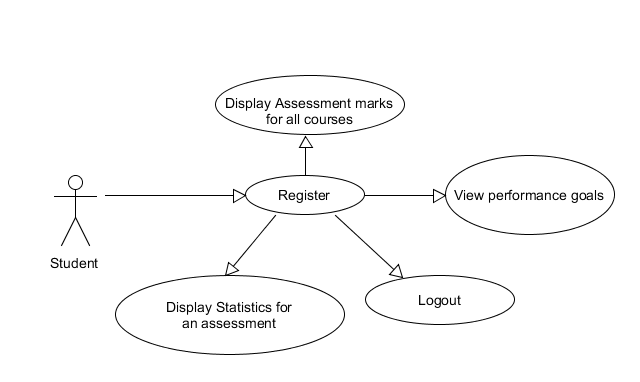
\includegraphics[trim={0cm 0cm 0cm 0cm },clip,scale = 1.1]{StudentUsecase}
			\caption{Use Case Diagram For Student}
		\end{figure}
	\end{center}
	
	
	
	\begin{center}
		\begin{tabular}{ | p{3cm} | p{10cm}| }
			\hline
			\textbf{Use case}& \textbf{Description} \\ \hline
			Register & The student need to sign in in order to view the results \\ \hline
			Display assessment marks & A student must be to display assessment marks for all courses  \\ \hline
			Statistics for an assessment & A student must be able to display assessment marks for a course and the statistics for that assessment \\ \hline
			View performance goals & A student must be able to view what perfomance goals are needed to pass pass the course based on current assessment \\ \hline
			Logout          & The student must be able to logout  \\ \hline
			
		\end{tabular}
	\end{center}
	\clearpage
	\subsubsection{Course Coordinator Use-Case Report}$\;\;\;\;\;\;\;\;\;\;\;\;\;\;\;\;\;\;\;\;\;\;\;$
	
	A use case report for Course Coordinator is shown in Figure 3.
	\begin{center}
		\begin{figure}[h]
			\centering
			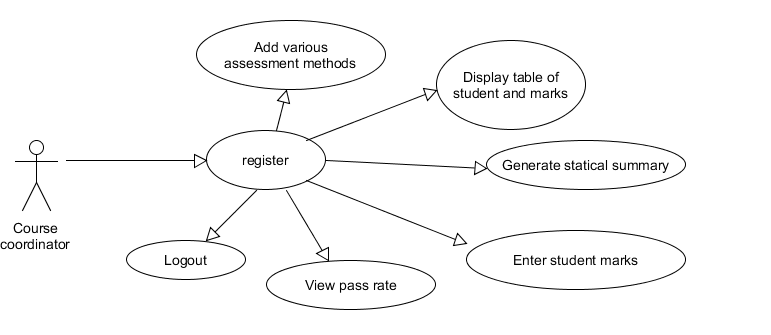
\includegraphics[trim={0cm 0cm 0cm 0cm },clip,scale = 0.85]{CourseCoordinatorUsecase}
			\caption{Use Case Diagram For Staff}
		\end{figure}
	\end{center}
	
	
	
	\begin{center}
		\begin{tabular}{ | p{3cm} | p{10cm}| }
			\hline
			\textbf{Use case}& \textbf{Description} \\ \hline
			Register & Staff need to sign in order to modify results \\ \hline
			Add various assessment methods & Add various assessment method for the course and the weighting for each assessment  \\ \hline
			
			Display table of student and marks & Display or print out the table
of studets and their marks\\ \hline
            Generate statical summary & Generate A summary statistics of the perfomance of each student  \\ \hline
            Enter student marks & Enters the student's marks for each assessment in a user-friendly interface \\ \hline
            View pass rate & View projected pass rate based on the assessment marks accumulated by the students in the class thus far \\ \hline
			Logout          & Coordinator member must be able to logout  \\ \hline
			
		\end{tabular}
	\end{center}
	
	
	
	
	\clearpage
	\subsubsection{Administrator Use-Case Report}$\;\;\;\;\;\;\;\;\;\;\;\;\;\;\;\;\;\;\;\;\;\;\;$
	
	A use case report for an Administrator is shown in Figure 4.
	\begin{center}
		\begin{figure}[h]
			\centering
			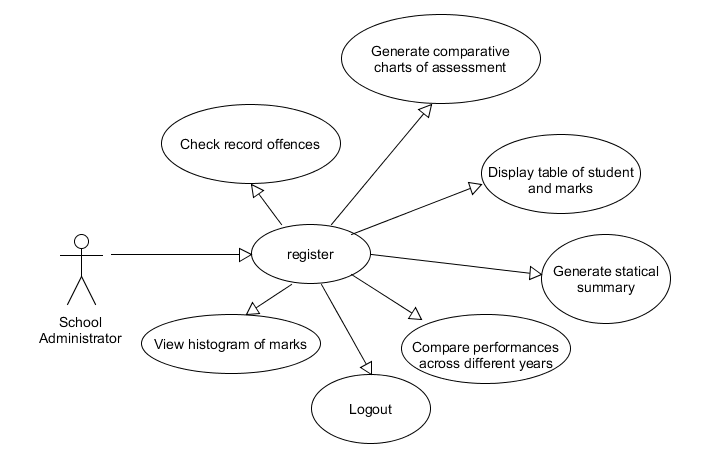
\includegraphics[trim={0cm 0cm 0cm 0cm },clip,scale = 0.85]{AdminUsecase}
			\caption{Use Case Diagram For Administrator}
		\end{figure}
	\end{center}
	
	
	
	\begin{center}
		\begin{tabular}{ | p{3cm} | p{10cm}| }
			\hline
			\textbf{Use case}& \textbf{Description} \\ \hline
			Register & Administrator need to sign in \\ \hline
			Check record offences & The administrator must be able to check any record offences like plagiarism for a student   \\ \hline
			Generate comparative charts of assessment & Generate a comparative chart of the assessment marks of selected courses 
being taken by students of a particular group \\ \hline
Display table of student and marks & Display or print out the table
of studets and their marks\\ \hline
Generate statical summary & Generate A summary statistics of the perfomance of each student  \\ \hline
Compare performances across different years & compare performances in the same course across different years \\ \hline 
View histogram of marks & View a histogram of assessment marks
of all courses taken by a specific specific student  \\ \hline 

			Logout          & Administrator must be able to logout  \\ \hline
			
		\end{tabular}
	\end{center}
	
	\newpage
	\section{Sequence Diagram}
	
	The sequence diagram in Figure 5 shows Sequence diagram of a student.  
	
	
	\begin{center}
		\begin{figure}[h]
			\centering
			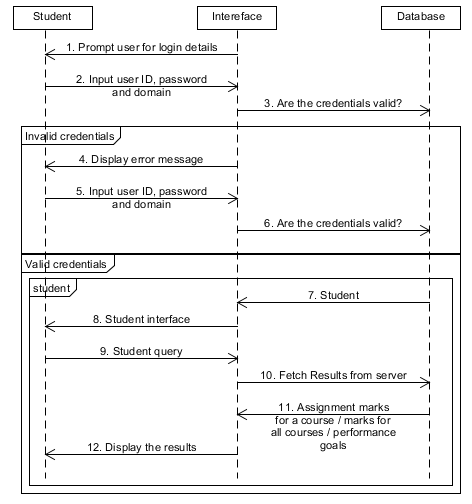
\includegraphics[trim={0cm 0cm 0cm 0cm },clip,scale = 1.3]{StudentSequence}
			\caption{Student Sequence Diagram}
		\end{figure}
	\end{center}
	\newpage
	
	
	The sequence diagram in Figure 6 shows Sequence diagram of an administrator.  
	
	
	\begin{center}
		\begin{figure}[h]
			\centering
			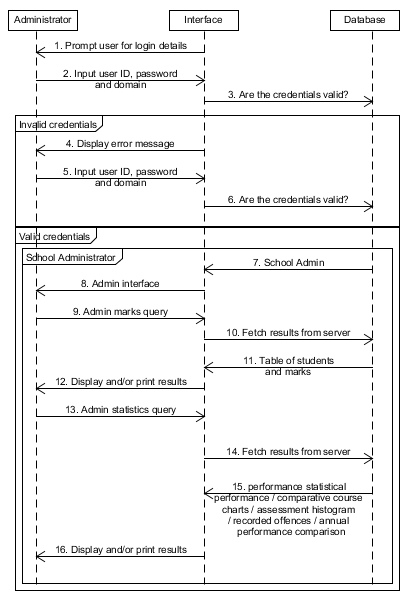
\includegraphics[trim={0cm 0cm 0cm 0cm },clip,scale = 1.1]{AdministratorSequence}
			\caption{ Administrator Sequence Diagram}
		\end{figure}
	\end{center}
	\newpage
	
		The sequence diagram in Figure 7 shows Sequence diagram of an course coordinator.  
	
	
	\begin{center}
		\begin{figure}[h]
			\centering
			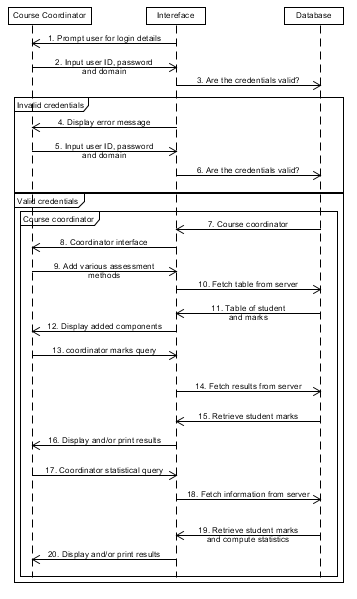
\includegraphics[trim={0cm 0cm 0cm 0cm },clip,scale = 1.1]{CoordinatorSequence}
			\caption{Course Coordinator Sequence Diagram}
		\end{figure}
	\end{center}

